%Corps du document :
%\setlength{\parindent}{1cm}    

\section{Conception détaillée}

Attachons nous maintenant à la conception détaille de notre application. Il s'agit
d'identifier et de spécifier les composants nécessaires pour automatiser tout ou
partie des outils à utiliser dans le cadre des cas d'utilisation identifiés.

Commençant par spécifier l'enchaînement des fenêtres grâce à un diagramme.

\subsection{Diagramme d'enchaînement des fenêtres}

\begin {center}
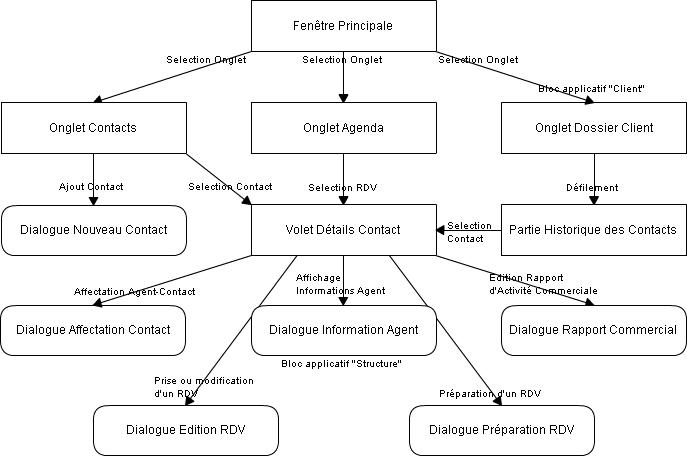
\includegraphics[width=\textwidth]{diagramme-edf.png}
\end {center}

\paragraph{Description}

L'Interface Homme-Machine (IHM) sera composée de trois onglets
principaux :

\begin{itemize}
\item \textbf{L'onglet Contacts} : Il présente la liste des Contacts prévus et affectés.
\item \textbf{L'onglet Agenda} : Il permet de consulter la liste des RDV pris.
\item \textbf{L'onglet Clients} : Cet onglet permet d'accéder aux dossiers des clients de la banque.
\end{itemize}

On observera également le volet \textbf{Détails du Contact}. Il permet d'effectuer toutes les
opérations nécessaires sur un Contact (une liste de ces services métiers se trouve plus loin
dans ce compte rendu).

\subsection{Dessin des fenêtres de l'IHM}

Voici une première représentation graphique de l'IHM que nous contruirons :

TODO @quentez

\subsection{Services Métiers invoqués par l'IHM}

Cette IHM utilise différents services métiers. En voici la liste :

\begin{itemize}
\item getAllClients()
\item afficherInfos(idClient)
\item updateClient(client)
\item getAllContacts(idAgence)
\item getAllAgents(idAgence)
\item affecterContactAgent(idAgent,idContact)
\item getContactsAgent(idAgent)
\item annulerContact(idContact,raison)
\item regrouperContacts(liste<Contact>)
\item planifierPlageAgenda(idAgent,typeActivite,date)
\item terminerPlanification()
\item getAgenda(type)
\item changerEtatContact(date,idContact,etat)
\item confirmerContact(lettre)
\item créerContactSpontané(date,idClient)
\item consulterCatalogue(idSegment,idProduit)
\item soumettreProposition(idContact,idOffre)
\item préparerContact(idContact)
\item consulterPréparation(idContact)
\item réaliserContact(idContact)
\item getSemaineParAgent(semaine,idAgent)
\item getJourAgence(date)
\item getPlageHoraire(idAgent,date)
\item transférerContact(idContact,idAgent)
\end{itemize}

\subsection{Spécification des Services Métier}

TODO @xsauvagnat

\subsection{Spécification des Services Objets Métier}

TODO @xsauvagnat

SOM 1 : getAllContacts
\begin{itemize}
\item Entrées : idAgence
\item Sorties : liste de (contact, nom du client, adresse client)
\item Entités/Classes : Client - Personne - Adresse - Contact
\item Permet de recuperer tous les contacts non assignés à un agent. Pour cela, la fonction récupère tous les clients de l'agence et verifie si un contact est prévu. 
\end{itemize}

SOM 2 : genererContactPrevu
\begin{itemize}
\item Entrées : evenement
\item Sorties : idClient
\item Entités/Classes : Evenement - Client
\item La fonction permet de récupérer l'id du client qui est à l'origine de l'évenement.
\end{itemize}
